Cada autovector que buscamos, proporciona nueva informaci\'on para nuestro an\'alisis. En esta secci\'on vamos a intentar ver cu\'al es esta informaci\'on, es decir, qu\'e es lo que nos est\'a diciendo cada autovector.

Vamos a tomar \'unicamente los primeros 3 autovectores obtenidos por cada m\'etodo, porque no se pueden graficar puntos en m\'as de 3 dimensiones.

\begin{table}[h!]
\begin{center}
\begin{tabular}{|c|c|c|}
	\hline
	\# & PCA & PLS-DA \\
	\hline
	Primer Autod\'igito &
	
\includegraphics[scale=4.00]{exp3/PCA-1} &
	
\includegraphics[scale=4.00]{exp3/PLS-1} \\
	\hline
	Segundo Autod\'igito &
	
\includegraphics[scale=4.00]{exp3/PCA-2} &
	
\includegraphics[scale=4.00]{exp3/PLS-2} \\
	\hline
	Tercer Autod\'igito &
	
\includegraphics[scale=4.00]{exp3/PCA-3} &
	
\includegraphics[scale=4.00]{exp3/PLS-3} \\
	\hline
\end{tabular}
\end{center}
\caption{Primeros autod\'igitos de los m\'etodos}
\end{table}

La tabla anterior muestra los 3 primeros autod\'igitos obtenidos para cada m\'etodo. Para obtener cada uno, se obtuvo el autovector asociado a cada uno de los primeros 3 autovalores, que est\'an normalizados. Se los convierte a base 0 - 1 \footnote{$(x^{i} - x_{min}) / (x_{max} - x_{min})$, con $x_{min}$ el m\'inimo valor encontrado en x y $x_{max}$ el m\'aximo, $x^{i}$ el $i$-\'esimo elemento de x} y se los multiplica por 255. As\'i obtenemos una matriz con valores entre 0 y 255 que representa una imagen, en particular la de los autod\'igitos.

\textbf{Hip\'otesis:} Dada la forma del primer autod\'igito, el primer autovector no admite confusi\'on entre los d\'igitos 0 y 1.

Para ver si esto vale, vamos a mostrar el extracto pertinente de las matrices de confusi\'on obtenidas para PCA y PLS-DA respectivamente:

\begin{table}[h!]
\begin{subtable}{.5\linewidth}
\begin{tabular}{|c|c|c|}
	\hline
	Actual\textbackslash Predicted & 0 & 1 \\
	\hline
	0 & 3009 & 0 \\
	\hline
	1 & 0 & 4091 \\
	\hline
\end{tabular}
\end{subtable}
\begin{subtable}{.5\linewidth}
\begin{tabular}{|c|c|c|}
	\hline
	Actual\textbackslash Predicted & 0 & 1 \\
	\hline
	0 & 3213 & 0 \\
	\hline
	1 & 0 & 3924 \\
	\hline
\end{tabular}
\end{subtable}
\end{table}

Se puede apreciar que la confusi\'on entre ambos d\'igitos es nula, el resto de la matriz no aporta grandes resultados, a excepci\'on que para el d\'igito 1:

Para PCA:

\begin{table}[h!]
\begin{tabular}{|c|c|c|c|c|c|c|c|c|c|c|}
	\hline
	Actual\textbackslash Predicted & 0 & 1 & 2 & 3 & 4 & 5 & 6 & 7 & 8 & 9 \\
	\hline
	1 & 0 & 3649 & 57 & 44 & 151 & 45 & 61 & 374 & 65 & 238 \\
	\hline
\end{tabular}
\end{table}

Para PLS-DA

\begin{table}[h!]
\begin{tabular}{|c|c|c|c|c|c|c|c|c|c|c|}
	\hline
	Actual\textbackslash Predicted & 0 & 1 & 2 & 3 & 4 & 5 & 6 & 7 & 8 & 9 \\
	\hline
	1 & 0 & 3924 & 8 & 25 & 91 & 7 & 7 & 421 & 24 & 177 \\
	\hline
\end{tabular}
\end{table}

Muestran que cuando la imagen a etiquetar es un 1, en la mayor\'ia de los casos va a acertar, pero si no lo hace, es m\'as probable que lo confunda con un 7 o con un 9, lo cual tiene sentido ya que los d\'igitos se parecen en su forma.

Es interesante entonces mostrar como se distribuyen los puntos en el nuevo espacio \footnote{El eje $y$ no es representativo, se tomo para simular $\mathbb{R}^{2}$}.

\begin{figure}[h!]
  \begin{center}
	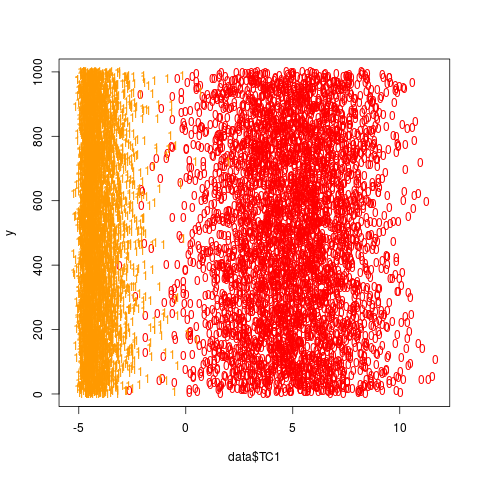
\includegraphics[scale=0.8]{exp5/PCA-1-0vs1}
	\caption{0 VS 1. Puntos en el nuevo espacio PCA}
  \end{center}
\end{figure}

\newpage

\begin{figure}[h!]
  \begin{center}
	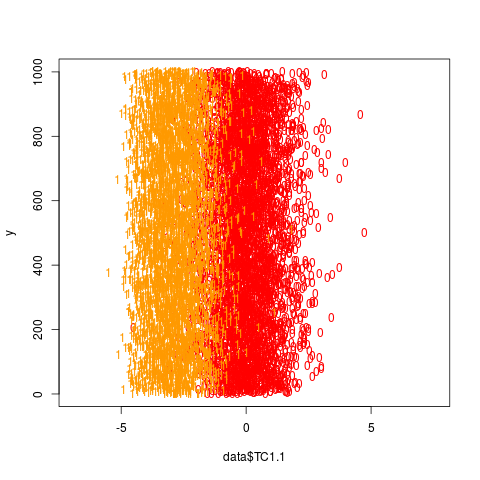
\includegraphics[scale=0.8]{exp5/PLS-1-0vs1}
	\caption{0 VS 1. Puntos en el nuevo espacio PLS-DA}
  \end{center}
\end{figure}

En PCA se ve una clara distancia entre los puntos transformados con etiquetas 0 y 1, guiados por el rasgo distintivo del autod\'igito. En PLS-DA parecer\'ia que se confunden en la frontera, aunque la mayor densidad de puntos est\'a en la media de cada uno, por lo que kNN clasificando un punto sobre la frontera no deber\'ia tener problemas \footnote{No pudimos encontrar una explicaci\'on para este fen\'omeno, creemos que la mayor\'ia de los 1's que se acercan a la media del 0 est\'an en la base de entrenamiento}.
